\documentclass[paper=a4, fontsize=12pt]{scrartcl} % A4 paper and 11pt font size

\usepackage[T1]{fontenc} % Use 8-bit encoding that has 256 glyphs
\usepackage[utf8]{inputenc} % Acentos
\usepackage{fourier} % Use the Adobe Utopia font for the document - comment this line to return to the LaTeX default
\usepackage{graphicx}
\usepackage{indentfirst}

\usepackage[inline]{enumitem} % inline enumerating
\usepackage{hyperref} 

\usepackage[brazil]{babel} % Portuguese Language

\usepackage{amsmath,amsfonts,amsthm} % Math packages

\usepackage{lipsum} % Used for inserting dummy 'Lorem ipsum' text into the template

\usepackage{sectsty} % Allows customizing section commands
\allsectionsfont{\centering \normalfont\scshape} % Make all sections centered, the default font and small caps

\usepackage{fancyhdr} % Custom headers and footers
\pagestyle{fancyplain} % Makes all pages in the document conform to the custom headers and footers
\fancyhead{} % No page header - if you want one, create it in the same way as the footers below
\fancyfoot[L]{} % Empty left footer
\fancyfoot[C]{} % Empty center footer
\fancyfoot[R]{\thepage} % Page numbering for right footer
\renewcommand{\headrulewidth}{0pt} % Remove header underlines
\renewcommand{\footrulewidth}{0pt} % Remove footer underlines
\setlength{\headheight}{13.6pt} % Customize the height of the header

\numberwithin{equation}{section} % Number equations within sections (i.e. 1.1, 1.2, 2.1, 2.2 instead of 1, 2, 3, 4)
\numberwithin{figure}{section} % Number figures within sections (i.e. 1.1, 1.2, 2.1, 2.2 instead of 1, 2, 3, 4)
\numberwithin{table}{section} % Number tables within sections (i.e. 1.1, 1.2, 2.1, 2.2 instead of 1, 2, 3, 4)

%\setlength\parindent{0pt} % Removes all indentation from paragraphs - comment this line for an assignment with lots of text

%----------------------------------------------------------------------------------------
%	TITLE SECTION
%----------------------------------------------------------------------------------------

\newcommand{\horrule}[1]{\rule{\linewidth}{#1}} % Create horizontal rule command with 1 argument of height

\title{	
\normalfont \normalsize 
\textsc{Universidade Federal do Rio de Janeiro} \\ [25pt] % Your university, school and/or department name(s)
\horrule{0.5pt} \\[0.4cm] % Thin top horizontal rule
\huge Linguagens de Programação \\
\huge Trabalho 3 \\ % The assignment title
\horrule{2pt} \\[0.5cm] % Thick bottom horizontal rule
}

\author{Aluno: Vinícius Aguiar Figueiredo \\
		Professor: Miguel Elias Mitre Campista} % Your name


\date{\normalsize\today} % Today's date or a custom date

\begin{document}

\maketitle % Print the title
\clearpage

\section{Introdução}

O programa desenvolvido possui por objetivo fornecer ao usuário uma
série de opções de validação de dados, retornando um ou mais arquivos
de texto que explicitam quais passaram e quais não passaram nos testes de validação. O programa foi desenvolvido utilizando-se das linguagens C++ e Perl.

\section{Implementação do Programa}

O programa principal é implementado de forma que o código em C++ seja o responsável por gerenciar as escolhas do usuário, dentre elas:
\begin{enumerate}
\item Qual tipo de dado para a validação usar (\textbf{5 opções disponíveis}, relatadas previamente, são eles CPF, CEP, Email, PlacaRJ e NumCel, cuja documentações e motivações já foram discutidas e elucidadas),
\item No caso de escolha do CPF, se haverá uso ou não de algoritmo extra,
\item Se serão validados apenas um ou múltiplos arquivos.
\end{enumerate}

O código em C++ portanto, chama através de 5 funções globais, subrotinas implementadas no código em Perl, tanto no código principal quanto nas dependências(módulos), utilizando-se da possibilidade de integração entre essas duas linguagens, documentada oficialmente como \href{https://perldoc.perl.org/perlembed.html}{\textit{perlembed}}.

No programa principal foi criada uma classe \textbf{Menu} capaz de permitir maior legibilidade ao código, assim como paradigmar o código à orientação de objetos.
Outra implementação do programa foi permitir ao usuário que selecione não apenas um, como no \textit{script} do 2º trabalho, mas sim múltiplos arquivos de texto para serem analisados de uma só vez. Neste contexto, foi utilizado o \textbf{std::vector}, STL Container do C++, assim como o \textbf{iterator} para realizar estas funções.


\section{O Programa em Uso}

O executável main (e os objects) são construídos utilizando-se o makefile incluso (\textit{\$ make}). 
Ao executar o script (\textit{\$ ./main}) o usuário é apresentado a um menu de opções, onde se espera que seja escolhida uma das análises de validação mostradas, o programa avisa ao usuário se o mesmo inserir uma opção inválida, e continua esperando uma válida. Ao ser escolhida uma opção válida, é pedido ao usuário que insira o nome do arquivo de texto a ser analisado. Neste momento, caso o usuário queira inserir mais de um, é apresentada a forma a ser inserida. Com a conclusão da análise o programa informa sobre o êxito da criação de um ou mais novos arquivos, que por padrão são chamados de \textit{modified + filename} e pergunta ao usuário se será feita uma outra análise ou se o mesmo deseja o encerramento do programa.

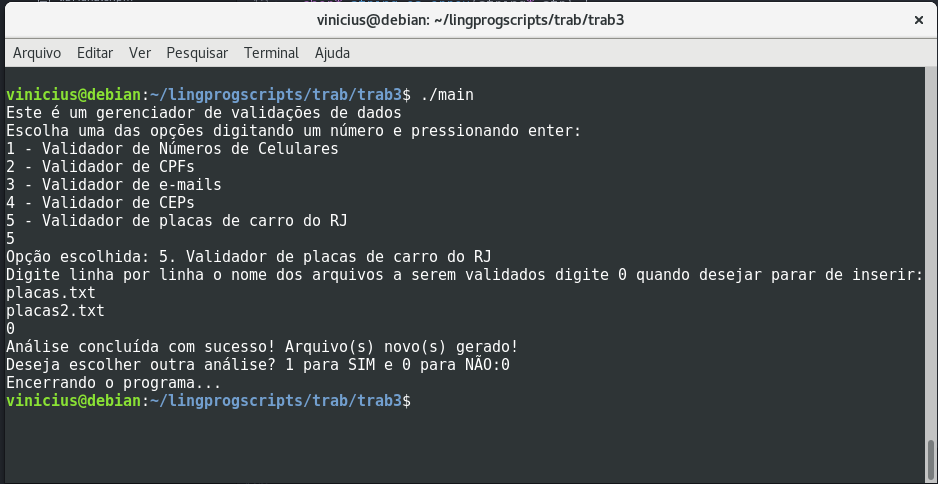
\includegraphics[scale=.6]{main.png}

Na imagem há um exemplo de execução do programa, sendo selecionada a opção 5., e dois arquivos de texto, placas.txt e placas2.txt. Os arquivos usados e outros estão inclusos na pasta do trabalho.

Na imagem abaixo, um exemplo de entrada e saída, mostrando também que há geração de arquivos de saída para cada arquivo de entrada (com o \textit{\$ ls}).

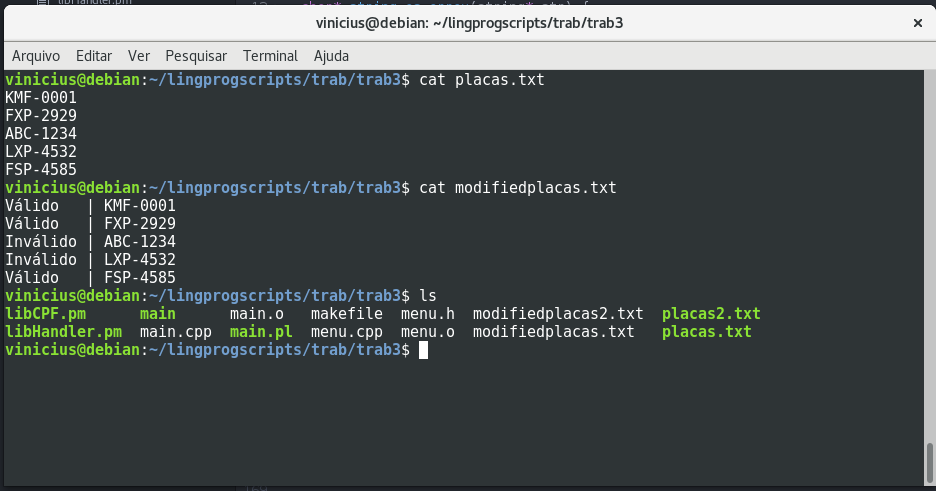
\includegraphics[scale=.6]{inout.png}

\section{Comentários e Conclusão}

Foram incluídos na pasta do trabalho todos os arquivos de texto usados para os testes das cinco funções. O programa cumpre bem o papel de gerenciador de validações e utiliza conceitos que tiram vantagem da \textit{Standard Library} do C++, como \textit{vectors}, \textit{strings} e \textit{iterators}. Há um incoveniente do usuário não poder usar a opção de múltiplas entradas na opção de validação de CPF, assim o fiz por permitir que o usuário especifique se quer ou não o uso do algoritmo em cada arquivo, separadamente. Apesar disto, o programa se comporta bem e cumpre de forma consistente o seu propósito. Para análise semântica e variações das regex, usei intensivamente o site \textit{https://regex101.com/}.


\end{document}
